% Options for packages loaded elsewhere
\PassOptionsToPackage{unicode}{hyperref}
\PassOptionsToPackage{hyphens}{url}
%
\documentclass[
]{article}
\usepackage{amsmath,amssymb}
\usepackage{lmodern}
\usepackage{iftex}
\ifPDFTeX
  \usepackage[T1]{fontenc}
  \usepackage[utf8]{inputenc}
  \usepackage{textcomp} % provide euro and other symbols
\else % if luatex or xetex
  \usepackage{unicode-math}
  \defaultfontfeatures{Scale=MatchLowercase}
  \defaultfontfeatures[\rmfamily]{Ligatures=TeX,Scale=1}
\fi
% Use upquote if available, for straight quotes in verbatim environments
\IfFileExists{upquote.sty}{\usepackage{upquote}}{}
\IfFileExists{microtype.sty}{% use microtype if available
  \usepackage[]{microtype}
  \UseMicrotypeSet[protrusion]{basicmath} % disable protrusion for tt fonts
}{}
\makeatletter
\@ifundefined{KOMAClassName}{% if non-KOMA class
  \IfFileExists{parskip.sty}{%
    \usepackage{parskip}
  }{% else
    \setlength{\parindent}{0pt}
    \setlength{\parskip}{6pt plus 2pt minus 1pt}}
}{% if KOMA class
  \KOMAoptions{parskip=half}}
\makeatother
\usepackage{xcolor}
\IfFileExists{xurl.sty}{\usepackage{xurl}}{} % add URL line breaks if available
\IfFileExists{bookmark.sty}{\usepackage{bookmark}}{\usepackage{hyperref}}
\hypersetup{
  pdftitle={Mendota\_timeseries},
  pdfauthor={Lauren A. Knose, ORISE-EPA},
  hidelinks,
  pdfcreator={LaTeX via pandoc}}
\urlstyle{same} % disable monospaced font for URLs
\usepackage[margin=1in]{geometry}
\usepackage{color}
\usepackage{fancyvrb}
\newcommand{\VerbBar}{|}
\newcommand{\VERB}{\Verb[commandchars=\\\{\}]}
\DefineVerbatimEnvironment{Highlighting}{Verbatim}{commandchars=\\\{\}}
% Add ',fontsize=\small' for more characters per line
\usepackage{framed}
\definecolor{shadecolor}{RGB}{248,248,248}
\newenvironment{Shaded}{\begin{snugshade}}{\end{snugshade}}
\newcommand{\AlertTok}[1]{\textcolor[rgb]{0.94,0.16,0.16}{#1}}
\newcommand{\AnnotationTok}[1]{\textcolor[rgb]{0.56,0.35,0.01}{\textbf{\textit{#1}}}}
\newcommand{\AttributeTok}[1]{\textcolor[rgb]{0.77,0.63,0.00}{#1}}
\newcommand{\BaseNTok}[1]{\textcolor[rgb]{0.00,0.00,0.81}{#1}}
\newcommand{\BuiltInTok}[1]{#1}
\newcommand{\CharTok}[1]{\textcolor[rgb]{0.31,0.60,0.02}{#1}}
\newcommand{\CommentTok}[1]{\textcolor[rgb]{0.56,0.35,0.01}{\textit{#1}}}
\newcommand{\CommentVarTok}[1]{\textcolor[rgb]{0.56,0.35,0.01}{\textbf{\textit{#1}}}}
\newcommand{\ConstantTok}[1]{\textcolor[rgb]{0.00,0.00,0.00}{#1}}
\newcommand{\ControlFlowTok}[1]{\textcolor[rgb]{0.13,0.29,0.53}{\textbf{#1}}}
\newcommand{\DataTypeTok}[1]{\textcolor[rgb]{0.13,0.29,0.53}{#1}}
\newcommand{\DecValTok}[1]{\textcolor[rgb]{0.00,0.00,0.81}{#1}}
\newcommand{\DocumentationTok}[1]{\textcolor[rgb]{0.56,0.35,0.01}{\textbf{\textit{#1}}}}
\newcommand{\ErrorTok}[1]{\textcolor[rgb]{0.64,0.00,0.00}{\textbf{#1}}}
\newcommand{\ExtensionTok}[1]{#1}
\newcommand{\FloatTok}[1]{\textcolor[rgb]{0.00,0.00,0.81}{#1}}
\newcommand{\FunctionTok}[1]{\textcolor[rgb]{0.00,0.00,0.00}{#1}}
\newcommand{\ImportTok}[1]{#1}
\newcommand{\InformationTok}[1]{\textcolor[rgb]{0.56,0.35,0.01}{\textbf{\textit{#1}}}}
\newcommand{\KeywordTok}[1]{\textcolor[rgb]{0.13,0.29,0.53}{\textbf{#1}}}
\newcommand{\NormalTok}[1]{#1}
\newcommand{\OperatorTok}[1]{\textcolor[rgb]{0.81,0.36,0.00}{\textbf{#1}}}
\newcommand{\OtherTok}[1]{\textcolor[rgb]{0.56,0.35,0.01}{#1}}
\newcommand{\PreprocessorTok}[1]{\textcolor[rgb]{0.56,0.35,0.01}{\textit{#1}}}
\newcommand{\RegionMarkerTok}[1]{#1}
\newcommand{\SpecialCharTok}[1]{\textcolor[rgb]{0.00,0.00,0.00}{#1}}
\newcommand{\SpecialStringTok}[1]{\textcolor[rgb]{0.31,0.60,0.02}{#1}}
\newcommand{\StringTok}[1]{\textcolor[rgb]{0.31,0.60,0.02}{#1}}
\newcommand{\VariableTok}[1]{\textcolor[rgb]{0.00,0.00,0.00}{#1}}
\newcommand{\VerbatimStringTok}[1]{\textcolor[rgb]{0.31,0.60,0.02}{#1}}
\newcommand{\WarningTok}[1]{\textcolor[rgb]{0.56,0.35,0.01}{\textbf{\textit{#1}}}}
\usepackage{graphicx}
\makeatletter
\def\maxwidth{\ifdim\Gin@nat@width>\linewidth\linewidth\else\Gin@nat@width\fi}
\def\maxheight{\ifdim\Gin@nat@height>\textheight\textheight\else\Gin@nat@height\fi}
\makeatother
% Scale images if necessary, so that they will not overflow the page
% margins by default, and it is still possible to overwrite the defaults
% using explicit options in \includegraphics[width, height, ...]{}
\setkeys{Gin}{width=\maxwidth,height=\maxheight,keepaspectratio}
% Set default figure placement to htbp
\makeatletter
\def\fps@figure{htbp}
\makeatother
\setlength{\emergencystretch}{3em} % prevent overfull lines
\providecommand{\tightlist}{%
  \setlength{\itemsep}{0pt}\setlength{\parskip}{0pt}}
\setcounter{secnumdepth}{-\maxdimen} % remove section numbering
\ifLuaTeX
  \usepackage{selnolig}  % disable illegal ligatures
\fi

\title{Mendota\_timeseries}
\author{Lauren A. Knose, ORISE-EPA}
\date{2023-05-02}

\begin{document}
\maketitle

The purpose of this program is to analyze the Mendota nutrient and water
quality data using time series analysis.

\hypertarget{step-1.-load-dependent-packages-and-data-needed}{%
\section{Step 1. Load dependent packages and data
needed:}\label{step-1.-load-dependent-packages-and-data-needed}}

\begin{enumerate}
\def\labelenumi{\alph{enumi})}
\tightlist
\item
  Loading dependent packages\ldots{}
\end{enumerate}

\begin{Shaded}
\begin{Highlighting}[]
\FunctionTok{library}\NormalTok{(ggplot2) }\CommentTok{\#needed for plots}
\FunctionTok{library}\NormalTok{(ggbreak) }\CommentTok{\#needed for plot scale breaks}
\end{Highlighting}
\end{Shaded}

\begin{verbatim}
## ggbreak v0.1.1
## 
## If you use ggbreak in published research, please cite the following
## paper:
## 
## S Xu, M Chen, T Feng, L Zhan, L Zhou, G Yu. Use ggbreak to effectively
## utilize plotting space to deal with large datasets and outliers.
## Frontiers in Genetics. 2021, 12:774846. doi: 10.3389/fgene.2021.774846
\end{verbatim}

\begin{Shaded}
\begin{Highlighting}[]
\FunctionTok{library}\NormalTok{(dplyr) }\CommentTok{\#needed for reshaping/reformaing data}
\end{Highlighting}
\end{Shaded}

\begin{verbatim}
## 
## Attaching package: 'dplyr'
\end{verbatim}

\begin{verbatim}
## The following objects are masked from 'package:stats':
## 
##     filter, lag
\end{verbatim}

\begin{verbatim}
## The following objects are masked from 'package:base':
## 
##     intersect, setdiff, setequal, union
\end{verbatim}

\begin{Shaded}
\begin{Highlighting}[]
\FunctionTok{library}\NormalTok{(lubridate) }\CommentTok{\#needed for date functions}
\end{Highlighting}
\end{Shaded}

\begin{verbatim}
## Loading required package: timechange
\end{verbatim}

\begin{verbatim}
## 
## Attaching package: 'lubridate'
\end{verbatim}

\begin{verbatim}
## The following objects are masked from 'package:base':
## 
##     date, intersect, setdiff, union
\end{verbatim}

\begin{Shaded}
\begin{Highlighting}[]
\FunctionTok{library}\NormalTok{(zoo) }\CommentTok{\#needed to interpolate data}
\end{Highlighting}
\end{Shaded}

\begin{verbatim}
## 
## Attaching package: 'zoo'
\end{verbatim}

\begin{verbatim}
## The following objects are masked from 'package:base':
## 
##     as.Date, as.Date.numeric
\end{verbatim}

\begin{Shaded}
\begin{Highlighting}[]
\FunctionTok{library}\NormalTok{(xts) }\CommentTok{\#needed to convert data frame to time series}
\end{Highlighting}
\end{Shaded}

\begin{verbatim}
## Warning: package 'xts' was built under R version 4.2.3
\end{verbatim}

\begin{verbatim}
## 
## ######################### Warning from 'xts' package ##########################
## #                                                                             #
## # The dplyr lag() function breaks how base R's lag() function is supposed to  #
## # work, which breaks lag(my_xts). Calls to lag(my_xts) that you type or       #
## # source() into this session won't work correctly.                            #
## #                                                                             #
## # Use stats::lag() to make sure you're not using dplyr::lag(), or you can add #
## # conflictRules('dplyr', exclude = 'lag') to your .Rprofile to stop           #
## # dplyr from breaking base R's lag() function.                                #
## #                                                                             #
## # Code in packages is not affected. It's protected by R's namespace mechanism #
## # Set `options(xts.warn_dplyr_breaks_lag = FALSE)` to suppress this warning.  #
## #                                                                             #
## ###############################################################################
\end{verbatim}

\begin{verbatim}
## 
## Attaching package: 'xts'
\end{verbatim}

\begin{verbatim}
## The following objects are masked from 'package:dplyr':
## 
##     first, last
\end{verbatim}

\begin{enumerate}
\def\labelenumi{\alph{enumi})}
\setcounter{enumi}{1}
\tightlist
\item
  Loading data\ldots{} Note, ensure date data is formatted in R as Date.
\end{enumerate}

\begin{Shaded}
\begin{Highlighting}[]
\NormalTok{Me\_P\_water}\OtherTok{\textless{}{-}} \FunctionTok{read.csv}\NormalTok{(}\AttributeTok{file=}\StringTok{"Cleaned\_data/Mendota\_P\_water.csv"}\NormalTok{)}
\NormalTok{Me\_P\_water}\OtherTok{\textless{}{-}}\NormalTok{ Me\_P\_water }\SpecialCharTok{\%\textgreater{}\%}
  \FunctionTok{mutate}\NormalTok{(}\AttributeTok{sampledate=}\FunctionTok{as.Date}\NormalTok{(sampledate, }\AttributeTok{origin=}\StringTok{"1899{-}12{-}30"}\NormalTok{), }\CommentTok{\#format as date}
         \AttributeTok{X=}\ConstantTok{NULL}\NormalTok{) }\CommentTok{\#remove extra column}
\NormalTok{Me\_Chla}\OtherTok{\textless{}{-}} \FunctionTok{read.csv}\NormalTok{(}\AttributeTok{file=}\StringTok{"Cleaned\_data/Mendota\_Chl.csv"}\NormalTok{)}
\NormalTok{Me\_Chla}\OtherTok{\textless{}{-}}\NormalTok{ Me\_Chla }\SpecialCharTok{\%\textgreater{}\%}
  \FunctionTok{mutate}\NormalTok{(}\AttributeTok{sampledate=}\FunctionTok{as.Date}\NormalTok{(sampledate, }\AttributeTok{origin=}\StringTok{"1899{-}12{-}30"}\NormalTok{), }\CommentTok{\#format as date}
         \AttributeTok{X=}\ConstantTok{NULL}\NormalTok{) }\CommentTok{\#remove extra column}
\NormalTok{Me\_Cyano}\OtherTok{\textless{}{-}} \FunctionTok{read.csv}\NormalTok{(}\AttributeTok{file=}\StringTok{"Cleaned\_data/Mendota\_Cyano.csv"}\NormalTok{)}
\NormalTok{Me\_Cyano}\OtherTok{\textless{}{-}}\NormalTok{ Me\_Cyano }\SpecialCharTok{\%\textgreater{}\%}
  \FunctionTok{mutate}\NormalTok{(}\AttributeTok{sampledate=}\FunctionTok{as.Date}\NormalTok{(sampledate, }\AttributeTok{origin=}\StringTok{"1899{-}12{-}30"}\NormalTok{), }\CommentTok{\#format as date}
         \AttributeTok{X=}\ConstantTok{NULL}\NormalTok{) }\CommentTok{\#remove extra column}
\NormalTok{Me\_P\_extinfl}\OtherTok{\textless{}{-}} \FunctionTok{read.csv}\NormalTok{(}\AttributeTok{file=}\StringTok{"Cleaned\_data/Mendota\_inflows.csv"}\NormalTok{)}
\NormalTok{Me\_P\_extinfl}\OtherTok{\textless{}{-}}\NormalTok{ Me\_P\_extinfl }\SpecialCharTok{\%\textgreater{}\%}
  \FunctionTok{mutate}\NormalTok{(}\AttributeTok{sampledate=}\FunctionTok{as.Date}\NormalTok{(sampledate, }\AttributeTok{origin=}\StringTok{"1899{-}12{-}30"}\NormalTok{), }\CommentTok{\#format as date}
         \AttributeTok{X=}\ConstantTok{NULL}\NormalTok{) }\CommentTok{\#remove extra column=as.Date(sampledate, orig))}
\end{Highlighting}
\end{Shaded}

\hypertarget{step-2.-combine-data-into-one-data-file}{%
\section{Step 2. Combine data into one data
file:}\label{step-2.-combine-data-into-one-data-file}}

\begin{enumerate}
\def\labelenumi{\alph{enumi})}
\tightlist
\item
  Merging nutrient data with Chl-a data by sample date\ldots{}
\end{enumerate}

\begin{Shaded}
\begin{Highlighting}[]
\NormalTok{Me\_Chla }\OtherTok{\textless{}{-}}\NormalTok{ Me\_Chla }\SpecialCharTok{\%\textgreater{}\%}
  \FunctionTok{mutate}\NormalTok{(}\AttributeTok{Yr=}\ConstantTok{NULL}\NormalTok{, }\AttributeTok{Mo=}\ConstantTok{NULL}\NormalTok{, }\AttributeTok{MoYr=}\ConstantTok{NULL}\NormalTok{, }\AttributeTok{daynum=}\ConstantTok{NULL}\NormalTok{) }\CommentTok{\#remove excess columns}
\NormalTok{water}\OtherTok{\textless{}{-}} \FunctionTok{merge}\NormalTok{(Me\_P\_water, Me\_Chla, }\AttributeTok{by=}\StringTok{"sampledate"}\NormalTok{)}
\end{Highlighting}
\end{Shaded}

Nutrient and Chl-a data merged.

\begin{enumerate}
\def\labelenumi{\alph{enumi})}
\setcounter{enumi}{1}
\tightlist
\item
  Merging nutrient data with Cyano data by sample date\ldots{}
\end{enumerate}

\begin{Shaded}
\begin{Highlighting}[]
\NormalTok{Me\_Cyano}\OtherTok{\textless{}{-}}\NormalTok{ Me\_Cyano }\SpecialCharTok{\%\textgreater{}\%}
  \FunctionTok{mutate}\NormalTok{(}\AttributeTok{Yr=}\ConstantTok{NULL}\NormalTok{, }\AttributeTok{Mo=}\ConstantTok{NULL}\NormalTok{, }\AttributeTok{MoYr=}\ConstantTok{NULL}\NormalTok{, }\AttributeTok{daynum=}\ConstantTok{NULL}\NormalTok{) }\CommentTok{\#remove excess columns}
\NormalTok{water}\OtherTok{\textless{}{-}} \FunctionTok{merge}\NormalTok{(water, Me\_Cyano, }\AttributeTok{by=}\StringTok{"sampledate"}\NormalTok{)}
\end{Highlighting}
\end{Shaded}

Nutrient and cyano data merged.

\begin{enumerate}
\def\labelenumi{\alph{enumi})}
\setcounter{enumi}{2}
\tightlist
\item
  Merging external loading with other data by sample date\ldots{}
\end{enumerate}

\begin{Shaded}
\begin{Highlighting}[]
\NormalTok{water}\OtherTok{\textless{}{-}} \FunctionTok{merge}\NormalTok{(water, Me\_P\_extinfl, }\AttributeTok{by=}\StringTok{"sampledate"}\NormalTok{)}
\end{Highlighting}
\end{Shaded}

\hypertarget{step-3.-view-data}{%
\section{Step 3. View data:}\label{step-3.-view-data}}

\begin{enumerate}
\def\labelenumi{\alph{enumi})}
\tightlist
\item
  plotting Hypo: Epi total P\ldots{}
\end{enumerate}

\begin{Shaded}
\begin{Highlighting}[]
\FunctionTok{ggplot}\NormalTok{(}\AttributeTok{data=}\FunctionTok{subset}\NormalTok{(water, }\FunctionTok{year}\NormalTok{(sampledate)}\SpecialCharTok{\textgreater{}} \DecValTok{2008}\NormalTok{), }\CommentTok{\#need to subset data because of big gap between 2000 and 2008}
       \FunctionTok{aes}\NormalTok{(}\AttributeTok{x=}\NormalTok{sampledate, }\AttributeTok{y=}\NormalTok{HE\_ratio\_TotP\_mgL)) }\SpecialCharTok{+}
  \FunctionTok{geom\_point}\NormalTok{() }\SpecialCharTok{+}
  \FunctionTok{geom\_line}\NormalTok{() }\SpecialCharTok{+} 
  \FunctionTok{theme\_classic}\NormalTok{() }\SpecialCharTok{+}
  \FunctionTok{labs}\NormalTok{(}\AttributeTok{x=}\StringTok{"Date"}\NormalTok{, }\AttributeTok{y=}\StringTok{"Hypo: Epi total P ratio"}\NormalTok{) }\SpecialCharTok{+}
  \FunctionTok{scale\_x\_date}\NormalTok{(}\AttributeTok{date\_breaks=}\StringTok{"1 year"}\NormalTok{) }
\end{Highlighting}
\end{Shaded}

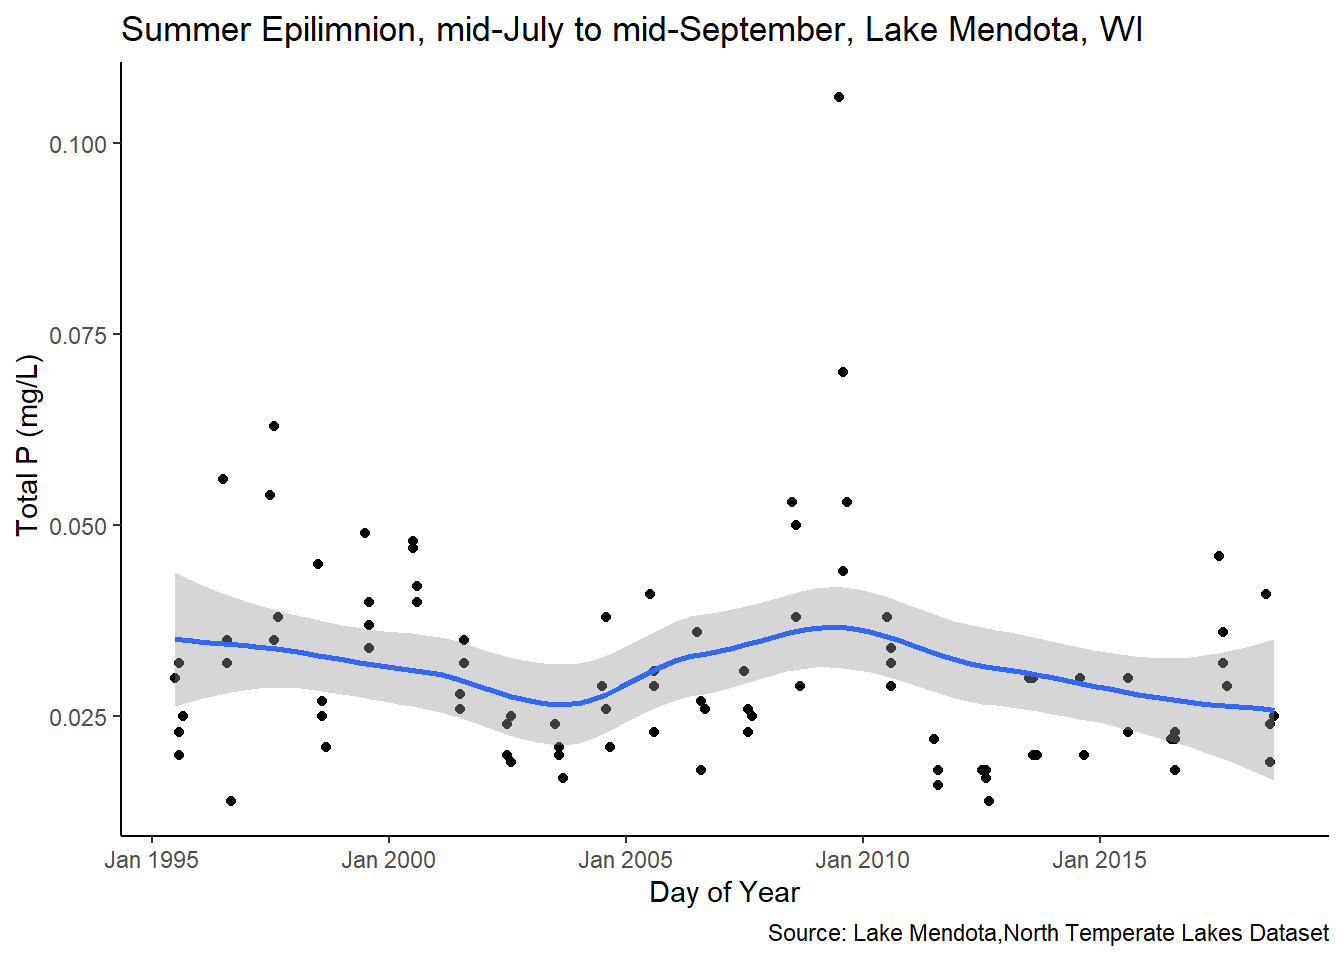
\includegraphics{Mendota_timeseries_files/figure-latex/unnamed-chunk-6-1.pdf}
Hypo: Epi total P ratio plotted.

\begin{enumerate}
\def\labelenumi{\alph{enumi})}
\setcounter{enumi}{1}
\tightlist
\item
  plotting chl-a\ldots{}
\end{enumerate}

\begin{Shaded}
\begin{Highlighting}[]
\FunctionTok{ggplot}\NormalTok{(}\AttributeTok{data=}\FunctionTok{subset}\NormalTok{(water, }\FunctionTok{year}\NormalTok{(sampledate)}\SpecialCharTok{\textgreater{}} \DecValTok{2008}\NormalTok{), }\CommentTok{\#need to subset data because of big gap between 2000 and 2008}
       \FunctionTok{aes}\NormalTok{(}\AttributeTok{x=}\NormalTok{sampledate,  }\AttributeTok{y=}\NormalTok{Chla\_ugL)) }\SpecialCharTok{+}
  \FunctionTok{geom\_point}\NormalTok{() }\SpecialCharTok{+}
  \FunctionTok{geom\_line}\NormalTok{() }\SpecialCharTok{+} 
  \FunctionTok{theme\_classic}\NormalTok{() }\SpecialCharTok{+}
  \FunctionTok{labs}\NormalTok{(}\AttributeTok{x=}\StringTok{"Date"}\NormalTok{, }\AttributeTok{y=}\StringTok{"Chlorophyll{-}a (ug/L)"}\NormalTok{) }\SpecialCharTok{+}
  \FunctionTok{scale\_x\_date}\NormalTok{(}\AttributeTok{date\_breaks=}\StringTok{"1 year"}\NormalTok{)}
\end{Highlighting}
\end{Shaded}

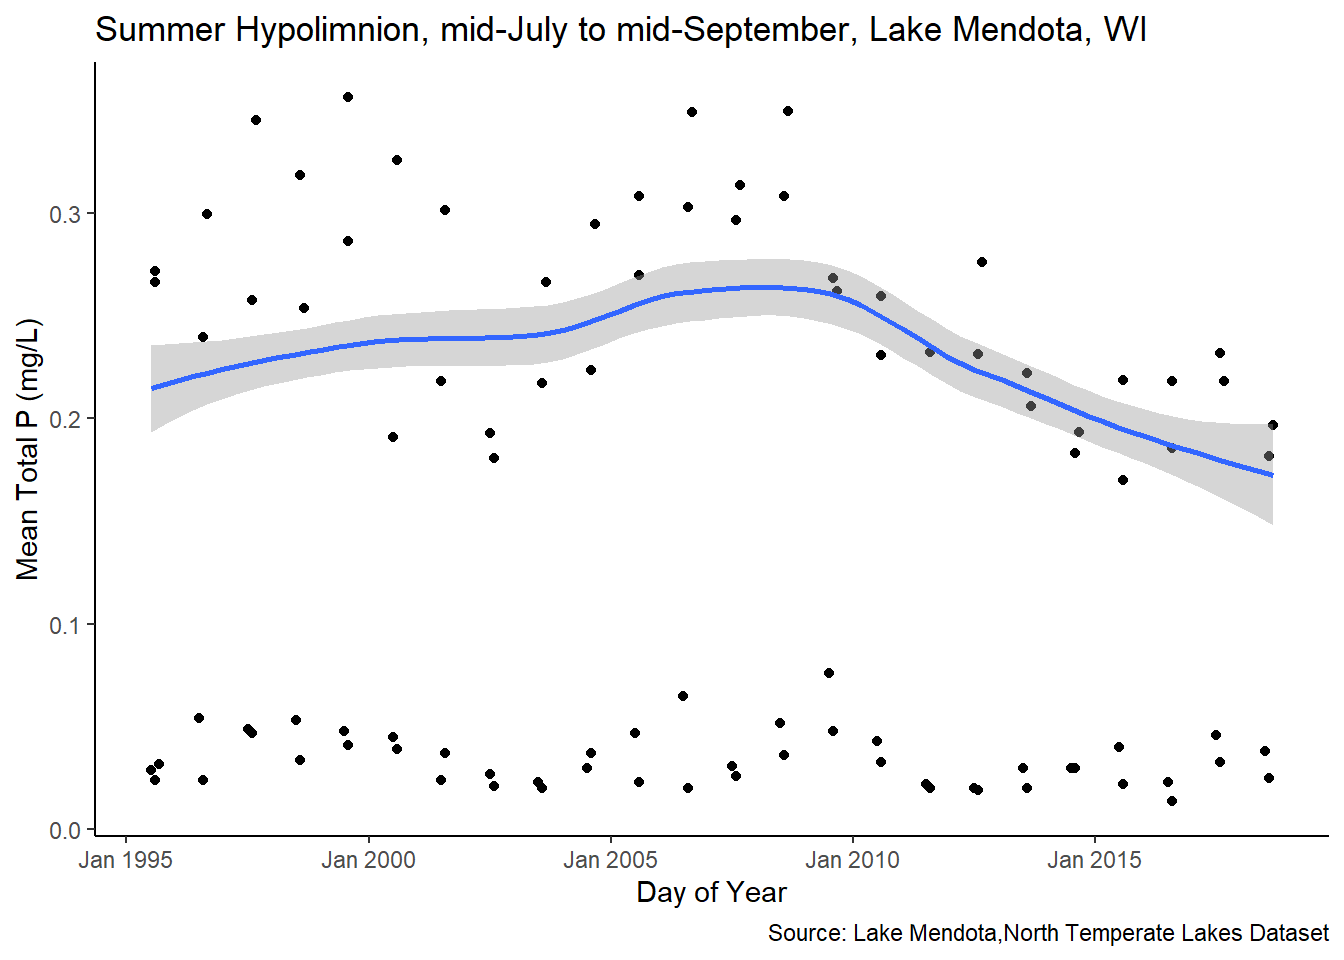
\includegraphics{Mendota_timeseries_files/figure-latex/unnamed-chunk-7-1.pdf}

Chl-a plotted.

\begin{enumerate}
\def\labelenumi{\alph{enumi})}
\setcounter{enumi}{2}
\tightlist
\item
  plotting Cyano relative biovolume\ldots{}
\end{enumerate}

\begin{Shaded}
\begin{Highlighting}[]
\FunctionTok{ggplot}\NormalTok{(}\AttributeTok{data=}\FunctionTok{subset}\NormalTok{(water, }\FunctionTok{year}\NormalTok{(sampledate)}\SpecialCharTok{\textgreater{}} \DecValTok{2008}\NormalTok{), }\CommentTok{\#need to subset data because of big gap between 2000 and 2008}
       \FunctionTok{aes}\NormalTok{(}\AttributeTok{x=}\NormalTok{sampledate,  }\AttributeTok{y=}\NormalTok{relbiovol)) }\SpecialCharTok{+}
  \FunctionTok{geom\_point}\NormalTok{() }\SpecialCharTok{+}
  \FunctionTok{geom\_line}\NormalTok{() }\SpecialCharTok{+} 
  \FunctionTok{theme\_classic}\NormalTok{() }\SpecialCharTok{+}
  \FunctionTok{labs}\NormalTok{(}\AttributeTok{x=}\StringTok{"Date"}\NormalTok{, }\AttributeTok{y=}\StringTok{"Cyanobacteria relative biovolume (as \% total algal)"}\NormalTok{) }\SpecialCharTok{+}
  \FunctionTok{scale\_x\_date}\NormalTok{(}\AttributeTok{date\_breaks=}\StringTok{"1 year"}\NormalTok{)}
\end{Highlighting}
\end{Shaded}

\includegraphics{Mendota_timeseries_files/figure-latex/unnamed-chunk-8-1.pdf}

Cyanobacteria relative biovolume plotted.

\begin{enumerate}
\def\labelenumi{\alph{enumi})}
\setcounter{enumi}{3}
\tightlist
\item
  plotting P external loading\ldots{}
\end{enumerate}

\begin{Shaded}
\begin{Highlighting}[]
\FunctionTok{ggplot}\NormalTok{(}\AttributeTok{data=}\FunctionTok{subset}\NormalTok{(water, }\FunctionTok{year}\NormalTok{(sampledate)}\SpecialCharTok{\textgreater{}} \DecValTok{2008}\NormalTok{), }\CommentTok{\#need to subset data because of big gap between 2000 and 2008}
       \FunctionTok{aes}\NormalTok{(}\AttributeTok{x=}\NormalTok{sampledate,  }\AttributeTok{y=}\NormalTok{TotP\_lbday\_sum)) }\SpecialCharTok{+}
  \FunctionTok{geom\_point}\NormalTok{() }\SpecialCharTok{+}
  \FunctionTok{geom\_line}\NormalTok{() }\SpecialCharTok{+} 
  \FunctionTok{theme\_classic}\NormalTok{() }\SpecialCharTok{+}
  \FunctionTok{labs}\NormalTok{(}\AttributeTok{x=}\StringTok{"Date"}\NormalTok{, }\AttributeTok{y=}\StringTok{"Total P external loading (lb/day)"}\NormalTok{) }\SpecialCharTok{+}
  \FunctionTok{scale\_x\_date}\NormalTok{(}\AttributeTok{date\_breaks=}\StringTok{"1 year"}\NormalTok{)}
\end{Highlighting}
\end{Shaded}

\includegraphics{Mendota_timeseries_files/figure-latex/unnamed-chunk-9-1.pdf}

\hypertarget{step-5.-transform-data-to-time-series}{%
\section{Step 5. Transform data to time
series:}\label{step-5.-transform-data-to-time-series}}

For time series, observations must be in equal time intervals. The
simplest practice is to model each variable over time and calculate the
predicted values for each observation. Use first order moving average
model (MA1) to interpolate missing observations (X\_t = u + w\_t +
theta\_1*w\_t-1).

\begin{enumerate}
\def\labelenumi{\alph{enumi})}
\tightlist
\item
  Hypo P: Epi P interpolation:
\end{enumerate}

\begin{Shaded}
\begin{Highlighting}[]
\NormalTok{date\_range}\OtherTok{\textless{}{-}} \FunctionTok{seq}\NormalTok{( }\CommentTok{\#creates a vector of sequence data}
  \FunctionTok{min}\NormalTok{(water}\SpecialCharTok{$}\NormalTok{sampledate), }\CommentTok{\#starting at the first sample date}
  \FunctionTok{max}\NormalTok{(water}\SpecialCharTok{$}\NormalTok{sampledate), }\CommentTok{\#ending at teh last sample date}
  \AttributeTok{by=}\StringTok{"14 days"}\NormalTok{) }\CommentTok{\#observations every 14 days (bimonthly) }
\NormalTok{interpolated}\OtherTok{\textless{}{-}} \FunctionTok{approx}\NormalTok{( }\CommentTok{\#creates a vector of data that linearly interpolates }
\NormalTok{  water}\SpecialCharTok{$}\NormalTok{sampledate, }\CommentTok{\#across date}
\NormalTok{  water}\SpecialCharTok{$}\NormalTok{HE\_ratio\_TotP\_mgL, }\CommentTok{\#the predicted values of Hypo P: Epi P ratio}
  \AttributeTok{xout=}\NormalTok{date\_range) }\CommentTok{\#for every 14 days}
\NormalTok{HEratio\_interp }\OtherTok{\textless{}{-}} \FunctionTok{data.frame}\NormalTok{( }\CommentTok{\#creates a new data frame that has }
  \AttributeTok{SampleDate =} \FunctionTok{as.Date}\NormalTok{(interpolated}\SpecialCharTok{$}\NormalTok{x), }\CommentTok{\#measurements every 14 days}
                             \AttributeTok{HE\_P\_ratio=}\NormalTok{interpolated}\SpecialCharTok{$}\NormalTok{y) }\CommentTok{\#predicted hypo: epi P ratio}
\FunctionTok{plot}\NormalTok{(HEratio\_interp,}
     \AttributeTok{xlab=}\StringTok{"Date"}\NormalTok{,}
     \AttributeTok{ylab=}\StringTok{"Hypo P: Epi P ratio"}\NormalTok{) }\CommentTok{\#plots the new time series}
\end{Highlighting}
\end{Shaded}

\includegraphics{Mendota_timeseries_files/figure-latex/unnamed-chunk-10-1.pdf}

Note there is a big data gap between 2000 and 2008, so we need to subset
the data to just post 2008.

\begin{Shaded}
\begin{Highlighting}[]
\FunctionTok{plot}\NormalTok{(}\FunctionTok{subset}\NormalTok{(HEratio\_interp, SampleDate }\SpecialCharTok{\textgreater{}=} \StringTok{"2008/1/1"}\NormalTok{),}
     \AttributeTok{xlab=}\StringTok{"Date"}\NormalTok{,}
     \AttributeTok{ylab=}\StringTok{"Hypo P: Epi P ratio"}\NormalTok{) }\CommentTok{\#plots the new time series}
\end{Highlighting}
\end{Shaded}

\includegraphics{Mendota_timeseries_files/figure-latex/unnamed-chunk-11-1.pdf}

\begin{enumerate}
\def\labelenumi{\alph{enumi})}
\setcounter{enumi}{1}
\tightlist
\item
  Chl-a interpolation:
\end{enumerate}

\begin{Shaded}
\begin{Highlighting}[]
\NormalTok{interpolated}\OtherTok{\textless{}{-}} \FunctionTok{approx}\NormalTok{( }\CommentTok{\#creates a vector of data that linearly interpolates }
\NormalTok{  water}\SpecialCharTok{$}\NormalTok{sampledate, }\CommentTok{\#across date}
\NormalTok{  water}\SpecialCharTok{$}\NormalTok{Chla\_ugL, }\CommentTok{\#the predicted values of Hypo P: Epi P ratio}
  \AttributeTok{xout=}\NormalTok{date\_range) }\CommentTok{\#for every 14 days}
\NormalTok{Chla\_interp }\OtherTok{\textless{}{-}} \FunctionTok{data.frame}\NormalTok{( }\CommentTok{\#creates a new data frame that has }
  \AttributeTok{SampleDate =} \FunctionTok{as.Date}\NormalTok{(interpolated}\SpecialCharTok{$}\NormalTok{x), }\CommentTok{\#measurements every 14 days}
                             \AttributeTok{Chla\_ugL=}\NormalTok{interpolated}\SpecialCharTok{$}\NormalTok{y) }\CommentTok{\#predicted hypo: epi P ratio}
\FunctionTok{plot}\NormalTok{(}\FunctionTok{subset}\NormalTok{(Chla\_interp, SampleDate }\SpecialCharTok{\textgreater{}=} \StringTok{"2008/1/1"}\NormalTok{),}
     \AttributeTok{xlab=}\StringTok{"Date"}\NormalTok{,}
     \AttributeTok{ylab=}\StringTok{"Total Chl{-}a (ugL)"}\NormalTok{) }\CommentTok{\#plots the new time series}
\end{Highlighting}
\end{Shaded}

\includegraphics{Mendota_timeseries_files/figure-latex/unnamed-chunk-12-1.pdf}

\begin{enumerate}
\def\labelenumi{\alph{enumi})}
\setcounter{enumi}{2}
\tightlist
\item
  Cyano rel biovol interpolation:
\end{enumerate}

\begin{Shaded}
\begin{Highlighting}[]
\NormalTok{interpolated}\OtherTok{\textless{}{-}} \FunctionTok{approx}\NormalTok{( }\CommentTok{\#creates a vector of data that linearly interpolates }
\NormalTok{  water}\SpecialCharTok{$}\NormalTok{sampledate, }\CommentTok{\#across date}
\NormalTok{  water}\SpecialCharTok{$}\NormalTok{relbiovol, }\CommentTok{\#the predicted values of Hypo P: Epi P ratio}
  \AttributeTok{xout=}\NormalTok{date\_range) }\CommentTok{\#for every 14 days}
\NormalTok{Cyan\_interp }\OtherTok{\textless{}{-}} \FunctionTok{data.frame}\NormalTok{( }\CommentTok{\#creates a new data frame that has }
  \AttributeTok{SampleDate =} \FunctionTok{as.Date}\NormalTok{(interpolated}\SpecialCharTok{$}\NormalTok{x), }\CommentTok{\#measurements every 14 days}
                             \AttributeTok{CRB=}\NormalTok{interpolated}\SpecialCharTok{$}\NormalTok{y) }\CommentTok{\#predicted hypo: epi P ratio}
\FunctionTok{plot}\NormalTok{(}\FunctionTok{subset}\NormalTok{(Cyan\_interp, SampleDate }\SpecialCharTok{\textgreater{}=} \StringTok{"2008/1/1"}\NormalTok{),}
     \AttributeTok{xlab=}\StringTok{"Date"}\NormalTok{,}
     \AttributeTok{ylab=}\StringTok{"Cyanobacteria Relative Biovolume (\% total)"}\NormalTok{) }\CommentTok{\#plots the new time series}
\end{Highlighting}
\end{Shaded}

\includegraphics{Mendota_timeseries_files/figure-latex/unnamed-chunk-13-1.pdf}

\begin{enumerate}
\def\labelenumi{\alph{enumi})}
\setcounter{enumi}{3}
\tightlist
\item
  total P external loading interpolation:
\end{enumerate}

\begin{Shaded}
\begin{Highlighting}[]
\NormalTok{interpolated}\OtherTok{\textless{}{-}} \FunctionTok{approx}\NormalTok{( }\CommentTok{\#creates a vector of data that linearly interpolates }
\NormalTok{  water}\SpecialCharTok{$}\NormalTok{sampledate, }\CommentTok{\#across date}
\NormalTok{  water}\SpecialCharTok{$}\NormalTok{TotP\_lbday\_sum, }\CommentTok{\#the predicted values of Hypo P: Epi P ratio}
  \AttributeTok{xout=}\NormalTok{date\_range) }\CommentTok{\#for every 14 days}
\NormalTok{ExtPload\_interp }\OtherTok{\textless{}{-}} \FunctionTok{data.frame}\NormalTok{( }\CommentTok{\#creates a new data frame that has }
  \AttributeTok{SampleDate =} \FunctionTok{as.Date}\NormalTok{(interpolated}\SpecialCharTok{$}\NormalTok{x), }\CommentTok{\#measurements every 14 days}
                             \AttributeTok{TotPextld\_lbday=}\NormalTok{interpolated}\SpecialCharTok{$}\NormalTok{y) }\CommentTok{\#predicted hypo: epi P ratio}
\FunctionTok{plot}\NormalTok{(}\FunctionTok{subset}\NormalTok{(ExtPload\_interp, SampleDate }\SpecialCharTok{\textgreater{}=} \StringTok{"2008/1/1"}\NormalTok{),}
     \AttributeTok{xlab=}\StringTok{"Date"}\NormalTok{,}
     \AttributeTok{ylab=}\StringTok{"Total P external load (lb/day)"}\NormalTok{) }\CommentTok{\#plots the new time series}
\end{Highlighting}
\end{Shaded}

\includegraphics{Mendota_timeseries_files/figure-latex/unnamed-chunk-14-1.pdf}

\hypertarget{step-6.-merge-all-time-series-into-single-data-frame-for-analysis}{%
\section{Step 6. Merge all time series into single data frame for
analysis:}\label{step-6.-merge-all-time-series-into-single-data-frame-for-analysis}}

\begin{Shaded}
\begin{Highlighting}[]
\NormalTok{water\_int}\OtherTok{\textless{}{-}} \FunctionTok{merge}\NormalTok{(Chla\_interp, Cyan\_interp, }\AttributeTok{by=}\StringTok{"SampleDate"}\NormalTok{)}
\NormalTok{water\_int}\OtherTok{\textless{}{-}} \FunctionTok{merge}\NormalTok{(water\_int, HEratio\_interp, }\AttributeTok{by=}\StringTok{"SampleDate"}\NormalTok{)}
\NormalTok{water\_int}\OtherTok{\textless{}{-}} \FunctionTok{merge}\NormalTok{(water\_int, ExtPload\_interp, }\AttributeTok{by=}\StringTok{"SampleDate"}\NormalTok{)}
\FunctionTok{write.csv}\NormalTok{(water\_int, }\AttributeTok{file=}\StringTok{"Cleaned\_data/Mendota\_ts.csv"}\NormalTok{)}
\end{Highlighting}
\end{Shaded}

All three data files merged.

\hypertarget{step-7.-perform-time-series-regression}{%
\section{Step 7. Perform time series
regression:}\label{step-7.-perform-time-series-regression}}

Time series regression model assumes the time series ``Y'' has a linear
relationship with the times series ``X''.

\begin{Shaded}
\begin{Highlighting}[]
\FunctionTok{hist}\NormalTok{(water\_int}\SpecialCharTok{$}\NormalTok{Chla\_ugL) }\CommentTok{\#prints histograph of Chl{-}a, log{-}transformed}
\end{Highlighting}
\end{Shaded}

\includegraphics{Mendota_timeseries_files/figure-latex/unnamed-chunk-16-1.pdf}

\begin{Shaded}
\begin{Highlighting}[]
\FunctionTok{hist}\NormalTok{(}\FunctionTok{lag}\NormalTok{(water\_int}\SpecialCharTok{$}\NormalTok{HE\_P\_ratio, }\AttributeTok{n=}\DecValTok{1}\NormalTok{)) }\CommentTok{\#prints histograph of P ratio, log10}
\end{Highlighting}
\end{Shaded}

\includegraphics{Mendota_timeseries_files/figure-latex/unnamed-chunk-16-2.pdf}

\begin{Shaded}
\begin{Highlighting}[]
\FunctionTok{hist}\NormalTok{(}\FunctionTok{lag}\NormalTok{(water\_int}\SpecialCharTok{$}\NormalTok{TotPextld\_lbday, }\AttributeTok{n=}\DecValTok{1}\NormalTok{))}\CommentTok{\#prints histograph of P external loading}
\end{Highlighting}
\end{Shaded}

\includegraphics{Mendota_timeseries_files/figure-latex/unnamed-chunk-16-3.pdf}

Need to transform both predictor and response variables to log 10, due
to skewness.

\begin{enumerate}
\def\labelenumi{\alph{enumi})}
\tightlist
\item
  Simplest model, glm: Chla\_t = hypoP:epiP\_t-k + error where k = 1
  Plot the response variable against the predictor to determine if
  linear or non-linear relationship.
\end{enumerate}

\begin{Shaded}
\begin{Highlighting}[]
\NormalTok{regk1}\OtherTok{\textless{}{-}} \FunctionTok{glm}\NormalTok{(}\FunctionTok{log10}\NormalTok{(water\_int}\SpecialCharTok{$}\NormalTok{Chla\_ugL}\FloatTok{+0.1}\NormalTok{)  }\SpecialCharTok{\textasciitilde{}} \CommentTok{\#response variable}
             \FunctionTok{lag}\NormalTok{(water\_int}\SpecialCharTok{$}\NormalTok{HE\_P\_ratio, }\AttributeTok{n=}\DecValTok{1}\NormalTok{)) }\CommentTok{\#X1 predictor variable}
\FunctionTok{summary}\NormalTok{(regk1)}
\end{Highlighting}
\end{Shaded}

\begin{verbatim}
## 
## Call:
## glm(formula = log10(water_int$Chla_ugL + 0.1) ~ lag(water_int$HE_P_ratio, 
##     n = 1))
## 
## Deviance Residuals: 
##     Min       1Q   Median       3Q      Max  
## -1.6258  -0.1231   0.1470   0.2892   0.7636  
## 
## Coefficients:
##                                   Estimate Std. Error t value Pr(>|t|)    
## (Intercept)                       0.630566   0.042274  14.916   <2e-16 ***
## lag(water_int$HE_P_ratio, n = 1) -0.002919   0.004174  -0.699    0.485    
## ---
## Signif. codes:  0 '***' 0.001 '**' 0.01 '*' 0.05 '.' 0.1 ' ' 1
## 
## (Dispersion parameter for gaussian family taken to be 0.2712541)
## 
##     Null deviance: 70.930  on 262  degrees of freedom
## Residual deviance: 70.797  on 261  degrees of freedom
##   (1 observation deleted due to missingness)
## AIC: 407.22
## 
## Number of Fisher Scoring iterations: 2
\end{verbatim}

\begin{Shaded}
\begin{Highlighting}[]
\FunctionTok{layout}\NormalTok{(}\FunctionTok{matrix}\NormalTok{(}\FunctionTok{c}\NormalTok{(}\DecValTok{1}\NormalTok{,}\DecValTok{2}\NormalTok{,}\DecValTok{3}\NormalTok{,}\DecValTok{4}\NormalTok{),}\DecValTok{2}\NormalTok{,}\DecValTok{2}\NormalTok{)) }\CommentTok{\# optional 4 graphs/page}
\FunctionTok{plot}\NormalTok{(regk1) }\CommentTok{\#prints diagnostic graphs for regression}
\end{Highlighting}
\end{Shaded}

\includegraphics{Mendota_timeseries_files/figure-latex/unnamed-chunk-17-1.pdf}

\begin{Shaded}
\begin{Highlighting}[]
\FunctionTok{par}\NormalTok{(}\AttributeTok{mfrow=}\FunctionTok{c}\NormalTok{(}\DecValTok{1}\NormalTok{,}\DecValTok{1}\NormalTok{))}
\end{Highlighting}
\end{Shaded}

\begin{enumerate}
\def\labelenumi{\alph{enumi})}
\setcounter{enumi}{1}
\tightlist
\item
  2nd model, glm: Chla\_t = hypoP:epiP\_t-k + Pexternalload\_t-k + error
  where k = 1 Plot the response variable against the predictor to
  determine if linear or non-linear relationship.
\end{enumerate}

\begin{Shaded}
\begin{Highlighting}[]
\NormalTok{regk2}\OtherTok{\textless{}{-}} \FunctionTok{glm}\NormalTok{(}\FunctionTok{log10}\NormalTok{(water\_int}\SpecialCharTok{$}\NormalTok{Chla\_ugL}\FloatTok{+0.1}\NormalTok{) }\SpecialCharTok{\textasciitilde{}} \CommentTok{\#response variable}
             \FunctionTok{lag}\NormalTok{(water\_int}\SpecialCharTok{$}\NormalTok{HE\_P\_ratio, }\AttributeTok{n=}\DecValTok{1}\NormalTok{) }\SpecialCharTok{+} \CommentTok{\#X1 predictor variable}
              \FunctionTok{lag}\NormalTok{(water\_int}\SpecialCharTok{$}\NormalTok{TotPextld\_lbday, }\AttributeTok{n=}\DecValTok{1}\NormalTok{)) }\CommentTok{\#X2 predictor variable}
\FunctionTok{summary}\NormalTok{(regk2)}
\end{Highlighting}
\end{Shaded}

\begin{verbatim}
## 
## Call:
## glm(formula = log10(water_int$Chla_ugL + 0.1) ~ lag(water_int$HE_P_ratio, 
##     n = 1) + lag(water_int$TotPextld_lbday, n = 1))
## 
## Deviance Residuals: 
##     Min       1Q   Median       3Q      Max  
## -1.6806  -0.1656   0.1154   0.3027   0.7782  
## 
## Coefficients:
##                                         Estimate Std. Error t value Pr(>|t|)
## (Intercept)                            0.7365905  0.0475929  15.477  < 2e-16
## lag(water_int$HE_P_ratio, n = 1)       0.0011170  0.0041422   0.270    0.788
## lag(water_int$TotPextld_lbday, n = 1) -0.0024625  0.0005656  -4.354 1.93e-05
##                                          
## (Intercept)                           ***
## lag(water_int$HE_P_ratio, n = 1)         
## lag(water_int$TotPextld_lbday, n = 1) ***
## ---
## Signif. codes:  0 '***' 0.001 '**' 0.01 '*' 0.05 '.' 0.1 ' ' 1
## 
## (Dispersion parameter for gaussian family taken to be 0.2537938)
## 
##     Null deviance: 70.930  on 262  degrees of freedom
## Residual deviance: 65.986  on 260  degrees of freedom
##   (1 observation deleted due to missingness)
## AIC: 390.71
## 
## Number of Fisher Scoring iterations: 2
\end{verbatim}

\begin{Shaded}
\begin{Highlighting}[]
\FunctionTok{layout}\NormalTok{(}\FunctionTok{matrix}\NormalTok{(}\FunctionTok{c}\NormalTok{(}\DecValTok{1}\NormalTok{,}\DecValTok{2}\NormalTok{,}\DecValTok{3}\NormalTok{,}\DecValTok{4}\NormalTok{),}\DecValTok{2}\NormalTok{,}\DecValTok{2}\NormalTok{)) }\CommentTok{\# optional 4 graphs/page}
\FunctionTok{plot}\NormalTok{(regk2) }\CommentTok{\#prints diagnostic graphs for regression}
\end{Highlighting}
\end{Shaded}

\includegraphics{Mendota_timeseries_files/figure-latex/unnamed-chunk-18-1.pdf}

\begin{Shaded}
\begin{Highlighting}[]
\FunctionTok{par}\NormalTok{(}\AttributeTok{mfrow=}\FunctionTok{c}\NormalTok{(}\DecValTok{1}\NormalTok{,}\DecValTok{1}\NormalTok{))}
\end{Highlighting}
\end{Shaded}

\begin{enumerate}
\def\labelenumi{\alph{enumi})}
\setcounter{enumi}{2}
\tightlist
\item
  3rd model, glm: Chla\_t = hypoP:epiP\_t-k + Pexternalload\_t-k +
  Chla\_t-k + error where k = 1 Plot the response variable against the
  predictor to determine if linear or non-linear relationship.
\end{enumerate}

\begin{Shaded}
\begin{Highlighting}[]
\NormalTok{regk3}\OtherTok{\textless{}{-}} \FunctionTok{glm}\NormalTok{(}\FunctionTok{log10}\NormalTok{(water\_int}\SpecialCharTok{$}\NormalTok{Chla\_ugL}\FloatTok{+0.1}\NormalTok{) }\SpecialCharTok{\textasciitilde{}} \CommentTok{\#response variable}
             \FunctionTok{lag}\NormalTok{(water\_int}\SpecialCharTok{$}\NormalTok{HE\_P\_ratio, }\AttributeTok{n=}\DecValTok{1}\NormalTok{) }\SpecialCharTok{+} \CommentTok{\#X1 predictor variable}
              \FunctionTok{lag}\NormalTok{(water\_int}\SpecialCharTok{$}\NormalTok{TotPextld\_lbday, }\AttributeTok{n=}\DecValTok{1}\NormalTok{) }\SpecialCharTok{+} \CommentTok{\#X2 predictor variable}
              \FunctionTok{lag}\NormalTok{(water\_int}\SpecialCharTok{$}\NormalTok{Chla\_ugL, }\AttributeTok{n=}\DecValTok{1}\NormalTok{)) }\CommentTok{\#X3 predictor variable}
\FunctionTok{summary}\NormalTok{(regk3)}
\end{Highlighting}
\end{Shaded}

\begin{verbatim}
## 
## Call:
## glm(formula = log10(water_int$Chla_ugL + 0.1) ~ lag(water_int$HE_P_ratio, 
##     n = 1) + lag(water_int$TotPextld_lbday, n = 1) + lag(water_int$Chla_ugL, 
##     n = 1))
## 
## Deviance Residuals: 
##      Min        1Q    Median        3Q       Max  
## -1.21472  -0.06622   0.09090   0.18256   0.63432  
## 
## Coefficients:
##                                         Estimate Std. Error t value Pr(>|t|)
## (Intercept)                            0.1467405  0.0465292   3.154  0.00180
## lag(water_int$HE_P_ratio, n = 1)       0.0074982  0.0028269   2.652  0.00848
## lag(water_int$TotPextld_lbday, n = 1) -0.0019539  0.0003839  -5.090  6.9e-07
## lag(water_int$Chla_ugL, n = 1)         0.0864575  0.0049216  17.567  < 2e-16
##                                          
## (Intercept)                           ** 
## lag(water_int$HE_P_ratio, n = 1)      ** 
## lag(water_int$TotPextld_lbday, n = 1) ***
## lag(water_int$Chla_ugL, n = 1)        ***
## ---
## Signif. codes:  0 '***' 0.001 '**' 0.01 '*' 0.05 '.' 0.1 ' ' 1
## 
## (Dispersion parameter for gaussian family taken to be 0.1162544)
## 
##     Null deviance: 70.93  on 262  degrees of freedom
## Residual deviance: 30.11  on 259  degrees of freedom
##   (1 observation deleted due to missingness)
## AIC: 186.36
## 
## Number of Fisher Scoring iterations: 2
\end{verbatim}

\begin{Shaded}
\begin{Highlighting}[]
\FunctionTok{anova}\NormalTok{(regk3)}
\end{Highlighting}
\end{Shaded}

\begin{verbatim}
## Analysis of Deviance Table
## 
## Model: gaussian, link: identity
## 
## Response: log10(water_int$Chla_ugL + 0.1)
## 
## Terms added sequentially (first to last)
## 
## 
##                                       Df Deviance Resid. Df Resid. Dev
## NULL                                                    262     70.930
## lag(water_int$HE_P_ratio, n = 1)       1    0.133       261     70.797
## lag(water_int$TotPextld_lbday, n = 1)  1    4.811       260     65.986
## lag(water_int$Chla_ugL, n = 1)         1   35.877       259     30.110
\end{verbatim}

\begin{Shaded}
\begin{Highlighting}[]
\FunctionTok{layout}\NormalTok{(}\FunctionTok{matrix}\NormalTok{(}\FunctionTok{c}\NormalTok{(}\DecValTok{1}\NormalTok{,}\DecValTok{2}\NormalTok{,}\DecValTok{3}\NormalTok{,}\DecValTok{4}\NormalTok{),}\DecValTok{2}\NormalTok{,}\DecValTok{2}\NormalTok{)) }\CommentTok{\# optional 4 graphs/page}
\FunctionTok{plot}\NormalTok{(regk3) }\CommentTok{\#prints diagnostic graphs for regression}
\end{Highlighting}
\end{Shaded}

\includegraphics{Mendota_timeseries_files/figure-latex/unnamed-chunk-19-1.pdf}

\begin{Shaded}
\begin{Highlighting}[]
\FunctionTok{par}\NormalTok{(}\AttributeTok{mfrow=}\FunctionTok{c}\NormalTok{(}\DecValTok{1}\NormalTok{,}\DecValTok{1}\NormalTok{))}
\end{Highlighting}
\end{Shaded}

\hypertarget{step-8.-compare-models}{%
\section{Step 8. Compare models:}\label{step-8.-compare-models}}

\begin{Shaded}
\begin{Highlighting}[]
\FunctionTok{anova}\NormalTok{(regk2, regk3) }\CommentTok{\#model with the lowest AIC offers better fit}
\end{Highlighting}
\end{Shaded}

\begin{verbatim}
## Analysis of Deviance Table
## 
## Model 1: log10(water_int$Chla_ugL + 0.1) ~ lag(water_int$HE_P_ratio, n = 1) + 
##     lag(water_int$TotPextld_lbday, n = 1)
## Model 2: log10(water_int$Chla_ugL + 0.1) ~ lag(water_int$HE_P_ratio, n = 1) + 
##     lag(water_int$TotPextld_lbday, n = 1) + lag(water_int$Chla_ugL, 
##     n = 1)
##   Resid. Df Resid. Dev Df Deviance
## 1       260     65.986            
## 2       259     30.110  1   35.877
\end{verbatim}

\hypertarget{step-9.-making-a-3d-plot}{%
\section{Step 9. Making a 3D plot}\label{step-9.-making-a-3d-plot}}

\begin{Shaded}
\begin{Highlighting}[]
\FunctionTok{library}\NormalTok{(rgl)}
\end{Highlighting}
\end{Shaded}

\begin{verbatim}
## Warning: package 'rgl' was built under R version 4.2.3
\end{verbatim}

\begin{Shaded}
\begin{Highlighting}[]
\NormalTok{water\_int}\OtherTok{\textless{}{-}} \FunctionTok{read.csv}\NormalTok{(}\AttributeTok{file=}\StringTok{"Cleaned\_data/Mendota\_ts.csv"}\NormalTok{)}
\end{Highlighting}
\end{Shaded}

\begin{Shaded}
\begin{Highlighting}[]
\NormalTok{mycols }\OtherTok{\textless{}{-}} \FunctionTok{colorRampPalette}\NormalTok{( }\FunctionTok{c}\NormalTok{(}\StringTok{"\#ff0000"}\NormalTok{, }\StringTok{"\#00ff00"}\NormalTok{) )}
\FunctionTok{plot3d}\NormalTok{( }
  \AttributeTok{x=}\NormalTok{water\_int}\SpecialCharTok{$}\StringTok{\textasciigrave{}}\AttributeTok{HE\_P\_ratio}\StringTok{\textasciigrave{}}\NormalTok{, }\AttributeTok{y=}\NormalTok{water\_int}\SpecialCharTok{$}\StringTok{\textasciigrave{}}\AttributeTok{TotPextld\_lbday}\StringTok{\textasciigrave{}}\NormalTok{, }\AttributeTok{z=}\FunctionTok{log10}\NormalTok{(water\_int}\SpecialCharTok{$}\StringTok{\textasciigrave{}}\AttributeTok{Chla\_ugL}\StringTok{\textasciigrave{}}\SpecialCharTok{+}\FloatTok{0.1}\NormalTok{), }
  \AttributeTok{colvar=}\NormalTok{water\_int}\SpecialCharTok{$}\NormalTok{Chla\_ugL,}
  \AttributeTok{type =} \StringTok{\textquotesingle{}s\textquotesingle{}}\NormalTok{, }
  \AttributeTok{radius =} \DecValTok{1}\NormalTok{,}
  \AttributeTok{xlab=}\StringTok{"Hypo: Epi P ratio"}\NormalTok{, }\AttributeTok{ylab=}\StringTok{"Total P external load (lb/day)"}\NormalTok{, }\AttributeTok{zlab=}\StringTok{"Total Chl{-}a (ug/L)"}\NormalTok{)}
\FunctionTok{rglwidget}\NormalTok{()}
\end{Highlighting}
\end{Shaded}

\begin{verbatim}
## Warning in snapshot3d(scene = x, width = width, height = height): webshot = TRUE
## requires the webshot2 package and Chrome browser; using rgl.snapshot() instead
\end{verbatim}

\includegraphics[width=6.5in]{../../../../../../../AppData/Local/Temp/Rtmpi8FDLe/file43b4163210dd}

\end{document}
